
Constructive heuristics and refinement heuristics  are often combined to form metaheuristic methods, which can be seen as general problem-solving frameworks that guide the search process by iteratively improving candidate solutions, as can be seen in Figure\ref{fig:metaheur}.

\begin{figure}[!h]
    \centering
    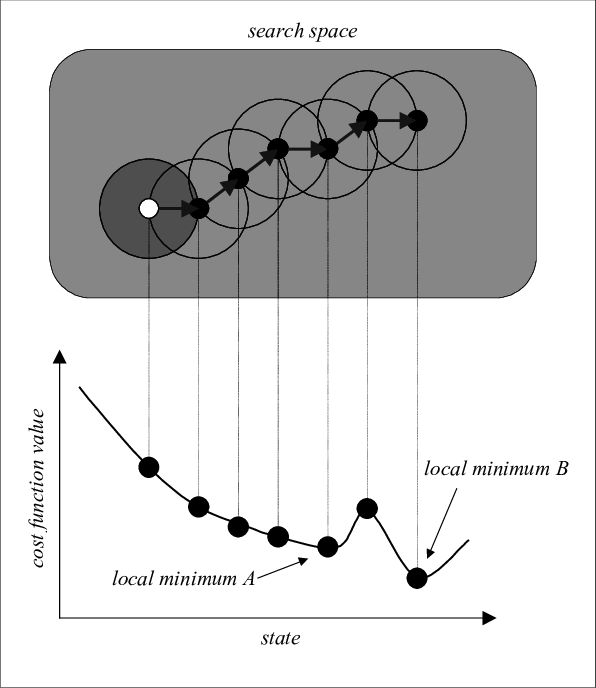
\includegraphics[]{images/metaheuristics.png}
    \caption{General behavior of a metaheuristic method}
    \label{fig:metaheur}
\end{figure}

Metaheuristic methods can be classified into two main categories: single-solution and population-based methods. Single-solution methods start with an initial solution and iteratively improve it by applying a set of moves or transformations. The single-solution metaheuristics that we implemented are Variable Neighborhood Search (VNS), Tabu Search and Simulated Annealing. Population-based methods maintain a population of candidate solutions and explore the search space by iteratively generating new solutions through genetic operators such as crossover and mutation. For the population-based methods we implemented a genetic Algorithm.





\section{Variable Neighborhood Search}
The Variable Neighborhood Search (VNS), proposed by Mladenović and Hansen in 1997,  is a metaheuristic optimization algorithm used to solve combinatorial optimization problems. The basic idea of VNS is to iteratively apply a perturbation operator to the current solution and then perform a local search around the perturbed solution. VNS is known for its flexibility and ability to escape from local optima by exploring different neighborhood structures.

In our implementation the VNS algorithm tries to improve the solution made by the 2-opt algorithm. In order to try to escape from the local minima produced by the 2-opt, the algorithm performs a random swap of 5 edges (called kick), see Figure \ref{fig:VNS} %%%


\begin{figure}[!h]
    \centering
    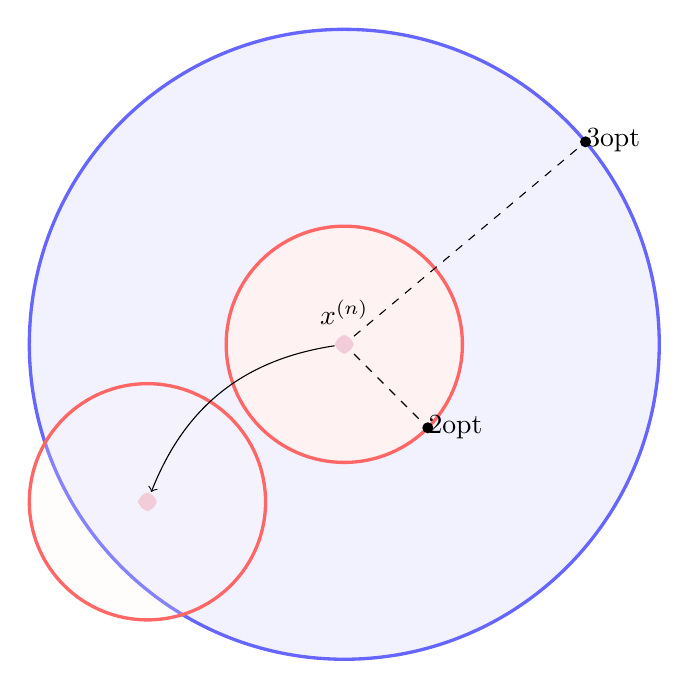
\begin{tikzpicture}
        \tikzstyle{city} = [fill=purple!20,rounded corners]
    

        \filldraw[color=blue!60, fill=blue!5, very thick](0,0) circle (4);

        \filldraw[color=red!60, fill=red!5, very thick](0,0) circle (1.5);

        \filldraw[color=red!60, fill=red!5, very thick, fill opacity=0.2](-2.5,-2) circle (1.5);

        
       
        \node[city,label=above:$x^{(n)}$] (A) at (0,0){};
        \node[city] (B) at (-2.5,-2){};

        

        \draw[->] (A) edge[bend right] node [right] {} (B);

        

        


        % define a random point (C) on this circle
        \path (0,0) ++(-45:1.5) coordinate (C);

        % draw (C) with a label
        \fill[black] (C) circle[radius=2pt] ++(1.5:1em) node {2opt};

        % define a random point (D) on this circle
        \path (0,0) ++(40:4) coordinate (D);

        % draw (C) with a label
        \fill[black] (D) circle[radius=2pt] ++(4:1em) node {3opt};
        

        \draw[dashed] (A) -- (C);
        \draw[dashed] (A) -- (D);




        %\draw[->] (0,0) arc (0:200:1.5);
       
    
    \end{tikzpicture}
    \caption{Example of VNS kick} \label{fig:VNS}
\end{figure}



Then it reapplies the 2-opt procedure and if it finds a better solution cost, it updates the global solution.
The overall procedure of Algorithm \ref{algo:VNS} is applied until a certain time limit is reached.
The algorithm requires $O(n)$ time for each kick, because after the swap operation we have to update the structure that contains all the nodes of the graph. We also have to sum the time required by the 2-opt algorithm. This time at the end has to be multiplied by the number of iterations that this procedure is performed. 

\begin{algorithm}[h!]
    \caption{VNS}\label{algo:VNS}
    \begin{algorithmic}[1]
    \Require $G = (V,E), c:E \to \mathbb{R}^+$
    \Ensure $\text{sub optimal TSP solution}$


    \State $solution \gets$ 2OPT(G)
   
   
    \While{$ !time\textunderscore expired$}
    \State kick(solution)   
    \State $ solution \gets $ 2OPT(solution)
    
    
    \If{cost(solution) < cost(best\textunderscore solution)}
    \State $ best\textunderscore solution \gets$ solution
    \EndIf
    

    \EndWhile

    \end{algorithmic}
\end{algorithm}

\subsection{Tuning of VNS}

\begin{figure}[!h]
    \centering
    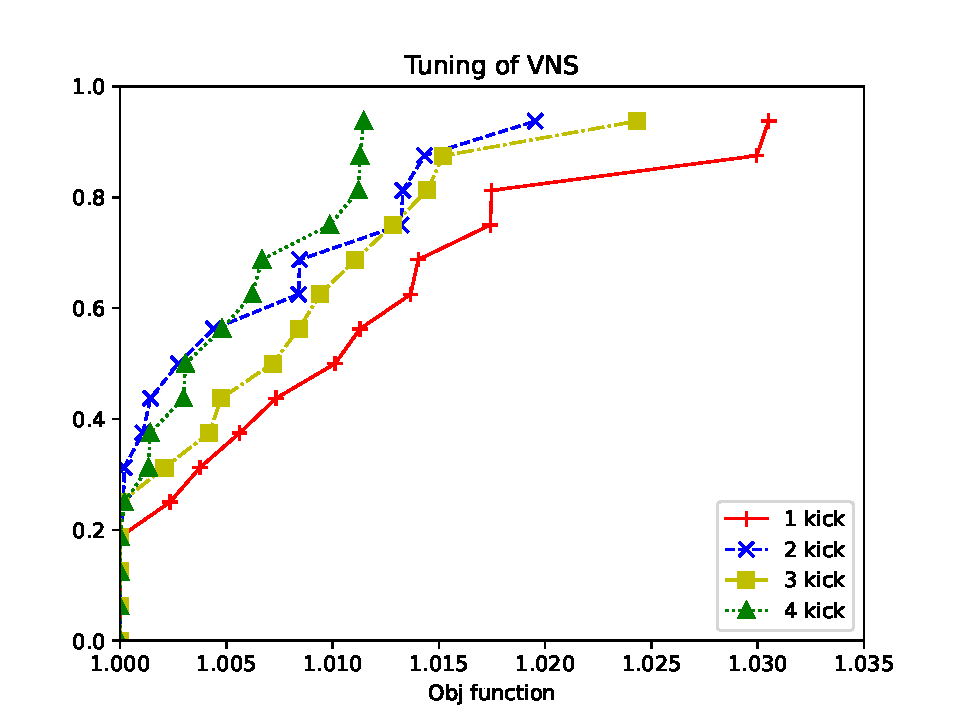
\includegraphics[width=\textwidth]{images/vns.pdf}
    \caption{VNS Tuning of number of kicks}
    \label{fig:vns}
\end{figure}

The VNS algorithm can vary its efficiency depending on how many kicks it computes at each iteration.

After some tests we noticed that the size of the instance didn't really affected the decision of how many kicks to make, so we made a comparison using the same number of kicks for each instance, disregarding its actual size, see Figure \ref{fig:vns}.





\section{Tabu Search}
Tabu search is a metaheuristic method created by Fred W. Glover in 1986.
It is based over the concept of "tabu" which means "prohibited" or "forbidden", following the idea that that the algorithm actually maintains a tabu list that keeps track of recent moves that are prohibited from being repeated. 
Tabu search is known for its ability to find good-quality solutions in a relatively short amount of time, although, as all other heuristic methods, it does not guarantee finding the optimal solution.

The algorithm starts with an initial solution, which can be generated randomly or by using a construction heuristic. In our implementation the initial solution is generated by the Greedy heuristic with the GRASP multistart variant, and optimized using the 2-opt algorithm.

At every iteration of the tabu algorithm, we select the pair of edges that have the minimum value of $\Delta$ (defined as in 2-opt, see Equation \ref{eq:delta}). Unike 2-opt algorithm, in Tabu Search doesn't matter if delta is negative or positive, we only take the minimum computed delta of the nodes that are not marked as “tabu” and then we select those nodes as candidate for a swap of edges (as in Figure\ref{fig:2OPT}).  After every swap, one of the four nodes involved is randomly select, and it is inserted into the “tabu” list.

The practice of using and updating a "tabu" list is used to prevent cycling, which means repeatedly visiting the same solutions over and over, without actually improving the current local optima. This allows the tabu method to diversify the search and explore different regions of the solution space. Thanks to this feature the algorithm moves around the solution space avoiding being stuck in local optima, and trying to find a better solution value, as can be seen in Figure \ref{fig:TABU}. This property can also be seen in practice, as in Figure \ref{fig:TABUPERF} where it is shown the possible output costs of the different solutions found by Tabu Search at each iteration.

\begin{figure}[!h]
    \centering
    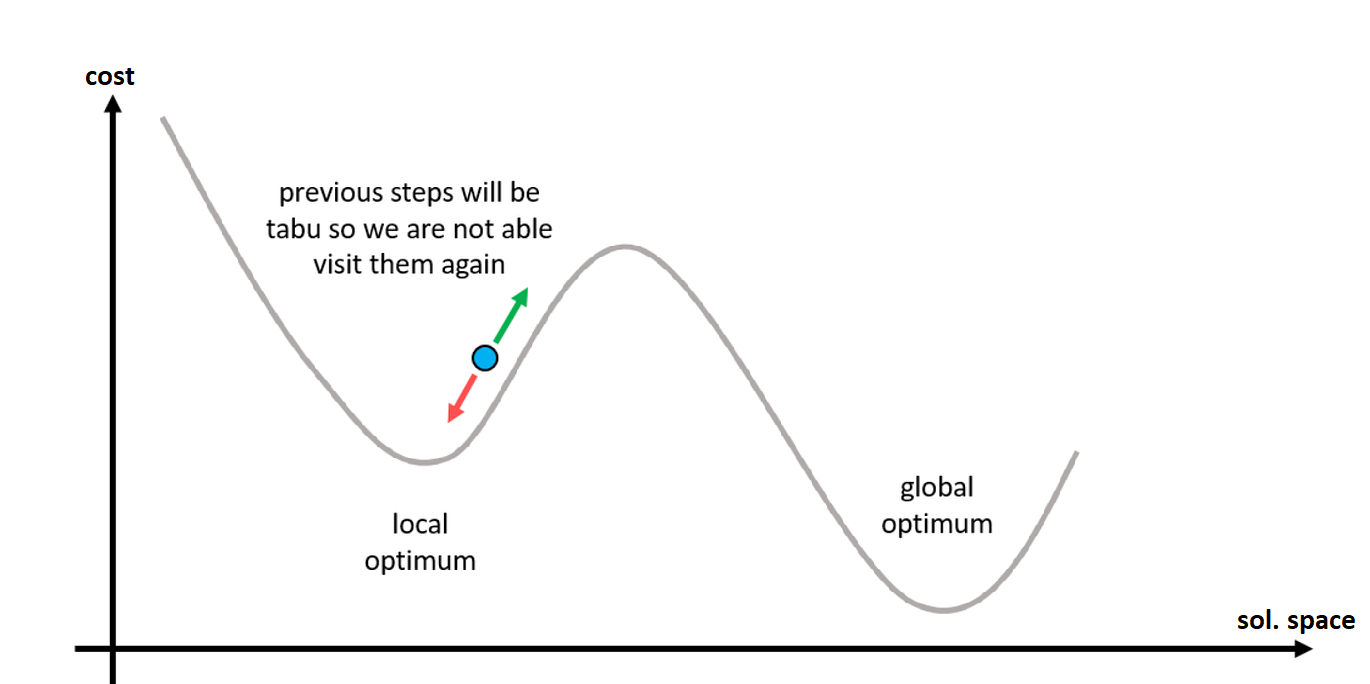
\includegraphics[width = \textwidth]{images/tabu.png}
    \caption{General behavior of a TABU method}
    \label{fig:TABU}
\end{figure}

\begin{figure}[!h]
    \centering
    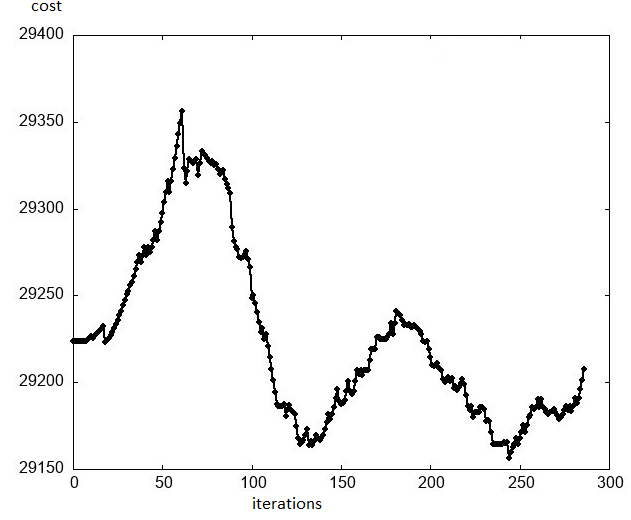
\includegraphics[scale=0.8]{images/tabuperf.png}
    \caption{progress of the objective function of tabu}
    \label{fig:TABUPERF}
\end{figure}

In order to implement the tabu list we create a list of length equals to the number of the nodes of the graph. Every time a node is selected to be a “tabu node” we set its corresponding element of the list equals to the number of the current iteration. Then this node cannot be involved in any swap operations until the number of the next iterations have overcome the value of a parameter called \textit{Tabu Tenure} that we saved as $T_{max}$, representing the number of iterations a node is forced to remain a "tabu" node and cannot be selected in a swap operation.
The value of $T_{max}$ is equivalent to the minimum between a \textit{Tabu Tenure} value and the number of nodes divided by the \textit{Tenure Ratio}, assuring that there are always nodes not labeled as forbidden and that can be used in the swap operation.

Each swap requires time equal to $O(n)$ to rearrange the array containing the actual solution. So the overall complexity of Algorithm \ref{algo:tabu} is equal to $O(n \cdot n_{swaps})$.
The algorithm stops after a given time limit returning in output the best solution found until then.

\begin{algorithm}[!h]
    \caption{Tabu}\label{algo:tabu}
    \begin{algorithmic}[1]
    \Require $G = (V,E), c:E \to \mathbb{R}^+$
    \Ensure $\text{sub optimal TSP solution}$


    \State $solution \gets$ 2OPT()
    \State $cost \gets$ cost\textunderscore 2OPT()
    \While{$ !time\textunderscore expired  $}
    \State $\Delta\gets$ $*$ best delta among all pairs of nodes that are not in the tabu list $*$
    \State $*$ choose a random node of delta and insert it into tabu list $*$
    \State $*$ updates tabu list $*$
    \State $edge\textunderscore 1 \gets$ new edge (a,b) that has to be inserted
    \State $edge\textunderscore 2 \gets$ new edge (b',a') that has to be inserted
    \State $swap(edge\textunderscore 1,edge\textunderscore 2) $
    \State $cost += \Delta$

    \If{cost < cost(best\textunderscore solution)}
    \State $ best\textunderscore solution \gets$ solution
    \State $ cost(best\textunderscore solution) \gets$ cost
    \EndIf
    

    \EndWhile

    \end{algorithmic}
\end{algorithm}



\begin{figure}[!h]
    \centering
    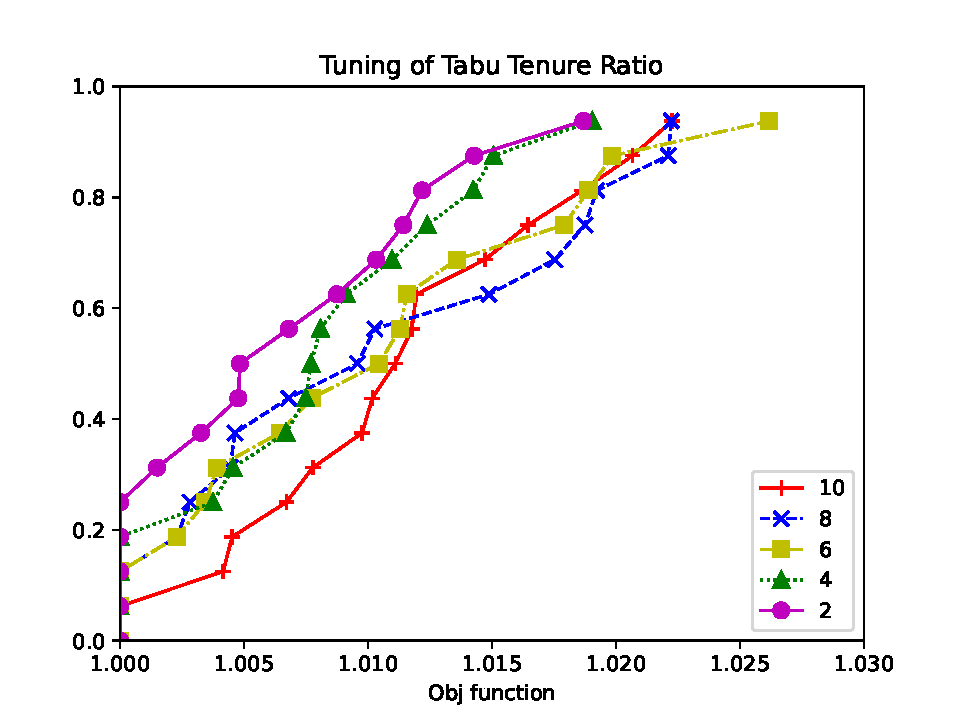
\includegraphics[width=\textwidth]{images/tabu.pdf}
    \caption{Tuning of Tabu Tenure Ratio}
    \label{fig:tabu}
\end{figure}
\subsection{Tuning of Tabu}

This section is used to identify and then tune the possible parameters that can alter the results of the Tabu Search algorithm.



The first parameter we tested is the \textit{Tenure Ratio}, a value that in our implementation serves the role of choosing the right \textit{Tenure} (or $T_{max}$) depending on the size of the input instance.

In Figure \ref{fig:tabu} we can see that a \textit{Tenure Ratio} of 2 has to be chosen to obtain the best performance on all the instances used.



The secondo parameter to be tested is the \textit{Tenure} itself. As an initial hypothesis we thought that having a bigger \textit{Tenure}, in the sense of forbidding certain moves for more time, could end up in finding better solutions, but Figure \ref{fig:tabu2} actually shows the opposite.

\begin{figure}[!h]
    \centering
    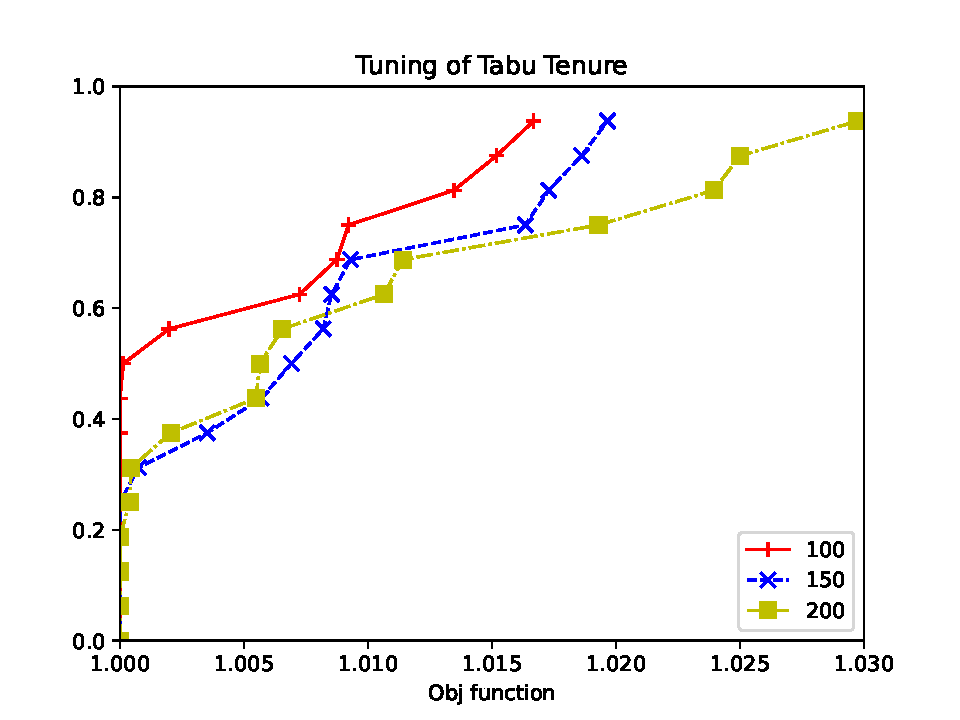
\includegraphics[width=\textwidth]{images/tabu2.pdf}
    \caption{Tuning of Tabu Tenure}
    \label{fig:tabu2}
\end{figure}


\section{Simulated Annealing}

Simulated Annealing is a metaheuristic optimization algorithm that can be used to solve the Travelling Salesman Problem (TSP).
The name of the algorithm comes from annealing in metallurgy, a technique involving heating and controlled cooling of a material to alter its physical properties. This method uses a probabilistic technique that usually archives an approximate solution of the global minimum.

Just like other metaheuristics, this algorithm starts with an initial solution, which can be generated randomly or using a heuristic. In our implementation we use the output of the Greedy heuristic with the GRASP and multistart variant as the initial solution that we want to improve.

At each iteration of the Algorithm \ref{algo:SimulatedAnnealing}, we select two edges $(a,a')$,$(b,b')$ randomly, where $a,a',b$ and $b'$ are distinct nodes and compute the $\Delta$ as in Equation \ref{eq:delta}. If there would be an improvement over the current solution, we swap the edges (as in Figure\ref{fig:2OPT} ). Else if the swap would result in the worsening of the solution, there is still a certain probability of making the swap anyway depending on a probability function over a parameter called Temperature. This method is actually an adaptation of the Metropolis algorithm published by Metropolis et al. in 1953 and the probability function used is defined as:



\begin{equation*}
    e^{\frac{-\Delta \operatorname{c}(a,b)}{T}}
\end{equation*}

\begin{algorithm}[!h]
    \caption{Simulated Annealing}\label{algo:SimulatedAnnealing}
    \begin{algorithmic}[1]
    \Require $G = (V,E), c:E \to \mathbb{R}^+$, a valid tour solution
    \Ensure $\text{sub optimal TSP solution}$

    \State cost $\gets$ cost(solution)

    \State $T \gets   T_0 $
    \State $ \alpha \gets  0.95 $
    \State $ iter \gets  0 $
   




    \While{$ !time\textunderscore expired$}
    

    \State $*$ Select two random edges and apply 2OPT move $*$

    
    \State $\Delta \gets *$ Difference of cost due to the 2OPT move $*$  
    
    
    \If{$\Delta \leq 0$}
    \State $*$ Update solution $*$
    \State cost $\gets$ cost + $\Delta$
    \Else 
    \State $*$ Update solution with probability $ e^{-\Delta \over T}*$

    \EndIf

    \State $T \gets T \cdot \alpha$
    \State $iter++ $
    \If{ $iter \geq$ 100}
    \State $T \gets   T_0$
    \State $iter \gets  $ 0
    \EndIf
    

    \EndWhile

    \end{algorithmic}
\end{algorithm}

where $T$ is called \textit{Temperature} and is computed over time as $T = \alpha \cdot T$, with $\alpha$ called \textit{cooling parameter} and starting with $T = T_0$ that actually depends on the input.

In our implementation of Algorithm \ref{algo:SimulatedAnnealing} the initial value for the temperature $T_0$ is equal to the cost of the input solution found by the GRASP Algorithm, divided by the number of nodes of the instance of the current TSP problem. Then at each iteration, $T$ is multiplied by the cooling parameter $\alpha = 0.95$. After 100 iterations of the algorithm, the temperature is newly set to its initial value $T_0$.

Each swap requires time equal to $O(n)$ to rearrange the array containing the actual solution. So the overall complexity is equal to $O(n \cdot number of swaps)$.
The algorithm stops its iteration after a given time limit.

	


\subsection{Tuning of Simulated Annealing}

To tune the probability used in the Simulated Annealing algorithm, the parameter to test is the \textit{cooling parameter} $\alpha$. Starting from the value of 0.99, we tested the range [0.95,0.99] to not have a too big decrease of $T$ at each iteration.

We can see in Figure \ref{fig:sa} that $\alpha = 0.95$ wins over the other values, for the only exception of $\alpha = 0.96$ in the higher percentiles.

\begin{figure}[!h]
    \centering
    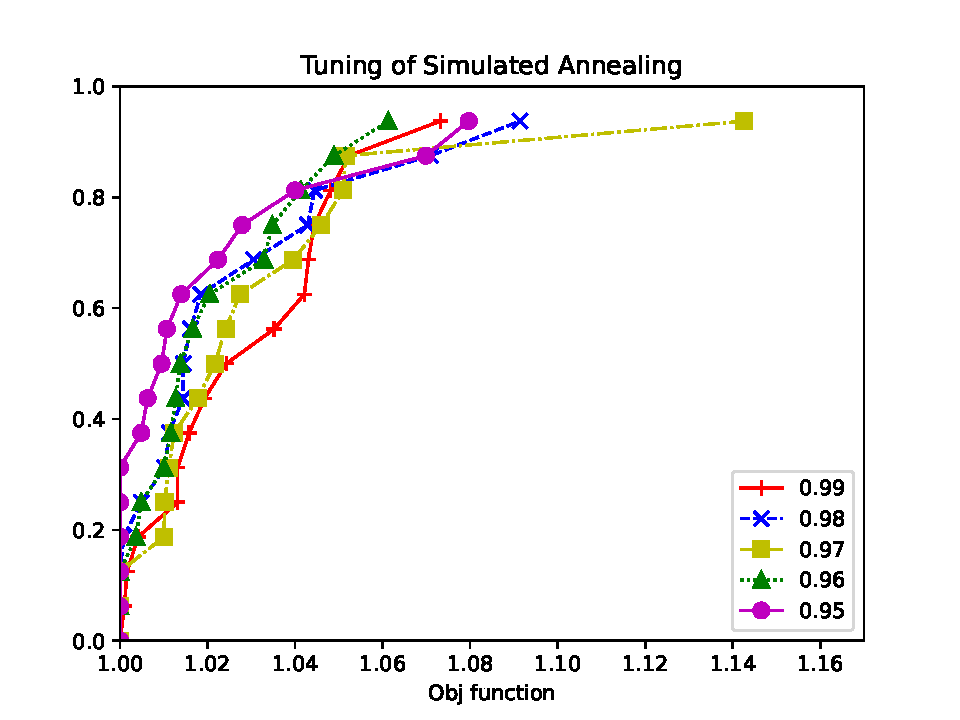
\includegraphics[width=\textwidth]{images/sa.pdf}
    \caption{Tuning of Simulated Annealing}
    \label{fig:sa}
\end{figure}

\section{genetic Algorithm}
Another approach to solving the TSP is to use a genetic Algorithm, which is a type of heuristic optimization algorithm inspired by the process of natural selection. genetic Algorithms work by creating an initial population of candidate solutions (called chromosomes), and then repeatedly applying genetic operators such as crossover and mutation to generate new, potentially better solutions, called offspring [\ref{algo:genetic}].


The choices of crossover and the chromosomes that make it to the next generation are based on the fitness of each chromosome, that is defined as minus the cost of the tsp tour. The genetic Algorithm then selects the fittest individuals to serve as parents for the next generation, with the hope that their good qualities will be passed on to their offspring.

To add some randomness in the hope of escaping the local optimums, a mutant is added with some probability to each new generation. A mutant is a chromosome of the current generation, chosen at random, to which a mutation has been applied, aka has some edges swapped at random.

Through this iterative process, the genetic Algorithm explores the space of possible solutions and gradually converges on a near-optimal tour.

In conclusion, the genetic Algorithm is a powerful and flexible approach to solving the Travelling Salesman Problem. While it may not always find the optimal solution, it can quickly find high-quality solutions that are good enough for many practical applications.

\begin{algorithm}
    \caption{genetic Algorithm}\label{algo:genetic}
    \begin{algorithmic}[1]
    \Require $G = (V,E), c:E \to \mathbb{R}^+$
    \Ensure $\text{sub optimal TSP solution}$
    
    \State $population \gets *$ initialize population of chromosomes using GRASP $*$

    \State $ generation \gets 0$

    \While{$generation < MAX \textunderscore GENERATION$}

        \State $parents \gets *$ initialize the offsparents  using a selection algorithm$*$
        \State $offspring \gets *$ initialize the offspring using crossover $*$

        \State $mutant \gets *$ if appropriate, initialize the mutant $*$

        \State $ newGeneration() $
        \State $ generation++ $

    \EndWhile

    \State $ solution \gets *$ chromosome with best fitness$*$

    

    \end{algorithmic}
\end{algorithm}

It's important to state elitism is implemented which means that the chromosomes with higher fitness (aka with lower cost) are always passed down to the next generation, ensuring that the best solution within all iterations of the genetic Algorithm is never killed. 

\subsubsection{Implementation choices}
There are several algorithms that can be used in conjunction with genetic Algorithm to enhance its performance.
During each iteration of the genetic Algorithm, selection, crossover and mutation are the main steps to compute to produce the new generation.
Selection algorithm determine which individuals from the current population should be chosen for reproduction to generate the next generation. The most commonly used selection algorithms are:

\begin{itemize}
    \item Roulette Wheel Selection: each chromosome in the population is assigned a probability of selection based on its fitness. The probabilities are proportional to the fitness of the individual, so that individuals with higher fitness have a higher chance of being selected. A random number is then generated, and the individual corresponding to the selected probability is chosen for reproduction. (It is the algorithm that we chose to implement in our project)
    \item Tournament Selection: a small subset of the population is randomly selected, and the individual with the highest fitness within that subset is chosen for reproduction.
\end{itemize}

After choosing two parents using selection, a new individual must be generated using a crossover algorithm. 
These algorithms determine how the tour information is exchanged between two parents during reproduction. Common crossover algorithms include single-point crossover, two-point crossover, and uniform crossover.
We implemented the single-point crossover and it works by choosing a single breaking point at random within the solutions of the parents and generating a partial new solution merging the chosen halves from the parents, without inserting duplicate nodes.
After that the new solution must be repaired and we chose to do so using the \ref{extramileage} Extra-Mileage Algorithm.

Mutation is computed within a certain probability and the chosen individual has its tour modified by the swapping of two random edges. Other common mutation algorithms include bit-flip mutation and inversion mutation.


\begin{figure}[!h]
    \centering
        %Prima riga
        \begin{subfigure}{0.48\textwidth} %Controllo della posizione in orizzontale
            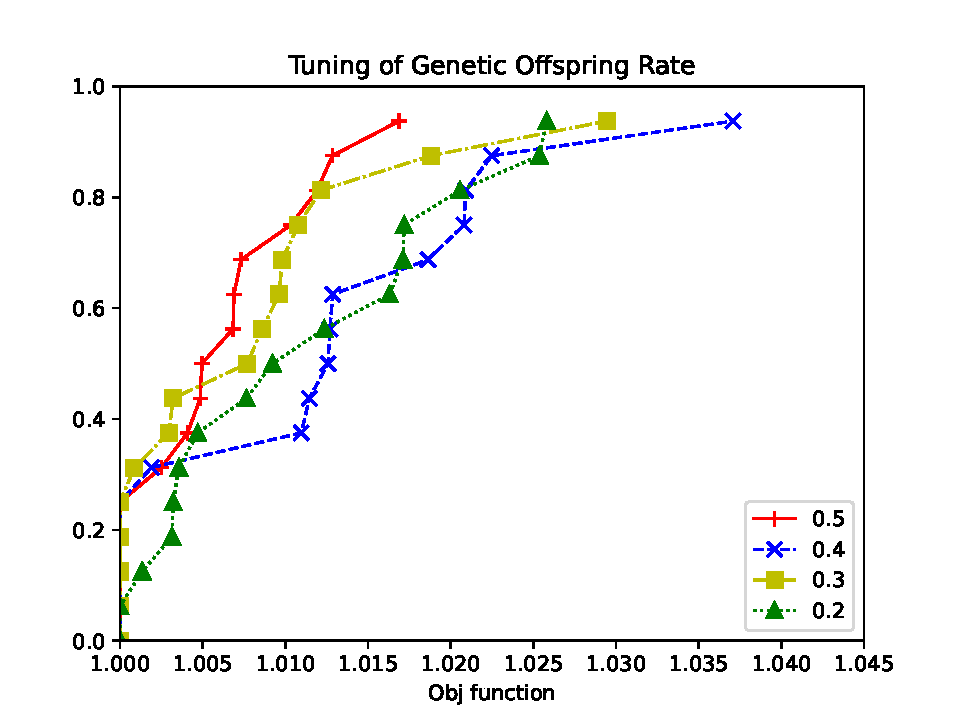
\includegraphics[scale=0.45]{images/genoff.pdf} 
            \caption{Tuning of Offspring Rate}
            \label{fig:genoff}
        \end{subfigure}
        \begin{subfigure}{0.48\textwidth}
            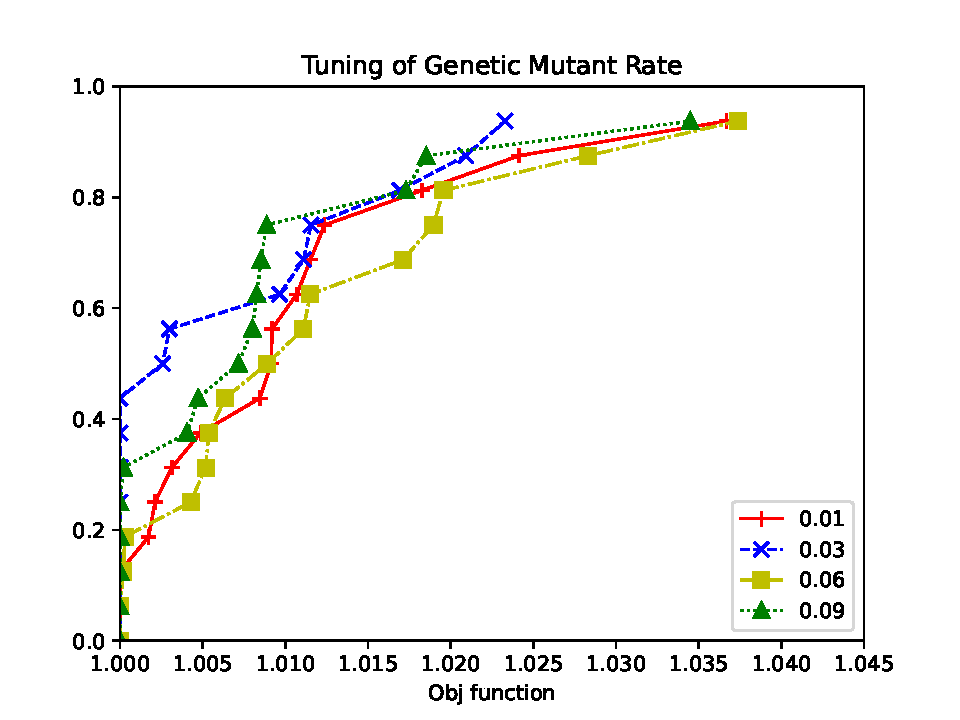
\includegraphics[scale=0.45]{images/genmut.pdf}
            \caption{Tuning of Mutant Rate}
            \label{fig:genmut}
        \end{subfigure}
    \caption{Tuning of the Genetic algorithm}
    \end{figure}

\subsection{Tuning of Genetic}

The most important parameters in the Genetic algorithm are the \textit{Offspring Rate} and the \textit{Mutant Rate}.

The \textit{Offspring Rate} determines the size of the new offspring generation based over a percentage of the size of the actual generation. This value changes the rate of finding possible better chromosomes, slowling or speeding up the process of natural selection.

In Figure \ref*{fig:genoff} can be seen that the values that compete the most are 0.5 and 0.3, but in the final implementation of the algorithm we chose \textit{Offspring Rate} = 0.5 since it performed better in the most cases.


The \textit{Mutant Rate} is tuned to add some well weighted randomness to the algorithm. Too many mutants can lead to worse possibilities of improvement, but a mutant is essential to assert a possibility of escapism from a possible local optima. 

We tested the range [0.1,0.9] to keep the probability of adding a mutant really low, and we can see in Figure \ref*{fig:genmut} that both 0.03 and 0.09 compete really well, but we chose to use a \textit{Mutant Rate} = 0.09.





\section{Comparison of Metaheuristic Algorithms}
This section is dedicated to the comparison of the Metaheuristic algorithms described above. 
It is important to highlight that these algorithms can vary its performance depending on their implementation, thus the results we are going to describe are intrinsically correct only within the boundaries of our own model.

In Figure \ref{fig:meta} we are comparing Tabu Search, VNS, Genetic and Simulated Annealing over the same instances, within the same time limit of 5 minutes, all of them with their corresponding tuned parameter, to assert the best possible performance.



\begin{figure}[!h]
    \centering
    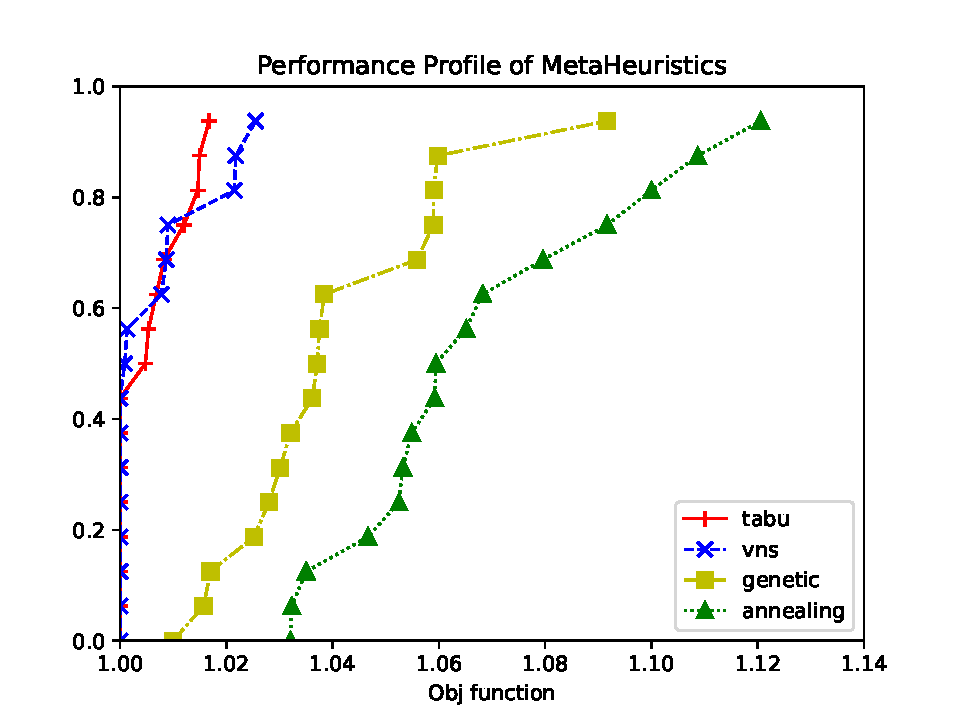
\includegraphics[width=\textwidth]{images/meta.pdf}
    \caption{Performance Profile of Metaheuristic algorithms}
    \label{fig:meta}
\end{figure}

\begin{table}[]
    \centering
    \begin{tabular}{lcccc}
    \cline{2-5}
                & \textbf{Tabu}   & \textbf{VNS}    & \textbf{Genetic} & \textbf{S. Annealing} \\ \hline
    att48.tsp   & 10611.110112    & 10625.430487    & 10995.308862     & 10983.016723       \\
    att532.tsp  & 29019.678235    & 28600.917059    & 30289.711639     & 29936.067989       \\
    d493.tsp    & 36979.874325    & 36370.285809    & 37735.484078     & 37545.598513       \\
    d657.tsp    & 51384.866148    & 50962.833321    & 54008.992502     & 54281.845932       \\
    dsj1000.tsp & 19803626.0 & 19821191.0 & 20114713.0  & 21618389.0  \\
    lin318.tsp  & 43502.354696    & 43270.515360    & 44658.919744     & 45646.363287       \\
    p654.tsp    & 34995.096723    & 35309.748105    & 35591.094654     & 39214.526200       \\
    pcb442.tsp  & 52965.274330    & 53426.635390    & 54301.288319     & 55783.711331       \\
    pr1002.tsp  & 268635.034053   & 274412.315655   & 293234.499257    & 295497.542051      \\
    pr439.tsp   & 110930.029029   & 109612.967166   & 112684.510372    & 118337.491854      \\
    rat575.tsp  & 7031.068022     & 7210.570174     & 7446.014269      & 7447.548178        \\
    rat783.tsp  & 9267.450174     & 9339.766424     & 9785.356566      & 9753.999949        \\
    rd400.tsp   & 16154.800276    & 16044.900084    & 16205.288761     & 16559.390143       \\
    u574.tsp    & 38885.965904    & 38700.991445    & 40137.238017     & 41341.810322       \\
    u724.tsp    & 44654.674979    & 43996.953223    & 45323.345043     & 46611.944462       \\
    vm1084.tsp  & 250014.164445   & 255459.278942   & 259630.598039    & 277195.165549      \\ \hline
    \end{tabular}
    \caption{Results of Metaheuristic Methods}
    \label{table:meta}
    \end{table}

    Data in Table \ref{table:meta} show the resulting values found running the Metaheuristic Algorithms over the relative instances. We can see that Tabu Search and VNS perform both really well, with Tabu being a little more precise over bigger instances. 








